%%%%%%%%%%%%%%%%%%%%%%%%%%%%%%%%%%%%%%%%%%%%%%%%%%%%%%%%%%%%%%%%%%%%%%%%%%%%%%%
% SECTION 5: Convolutional Neural Networks
%%%%%%%%%%%%%%%%%%%%%%%%%%%%%%%%%%%%%%%%%%%%%%%%%%%%%%%%%%%%%%%%%%%%%%%%%%%%%%%
\section{Convolutional Neural Networks}

% The Problem with Images
\begin{frame}{The Problem with Fully Connected Networks}
    \textbf{Applying standard networks to images:}
    
    \vspace{1em}
    \begin{itemize}
        \item A 256×256 RGB image = \textbf{\textasciitilde200,000 inputs}
        \item Fully connected to 1000 neurons = 200 million parameters in layer 1 alone
        \item No spatial awareness: pixel (0,0) and pixel (255,255) treated the same
        \item Small shifts break everything
    \end{itemize}
    
    \vspace{1em}
    \textbf{Unmanageable and fundamentally wrong approach}
\end{frame}

% CNN Structure
\begin{frame}{CNN Structure}
    \begin{center}
        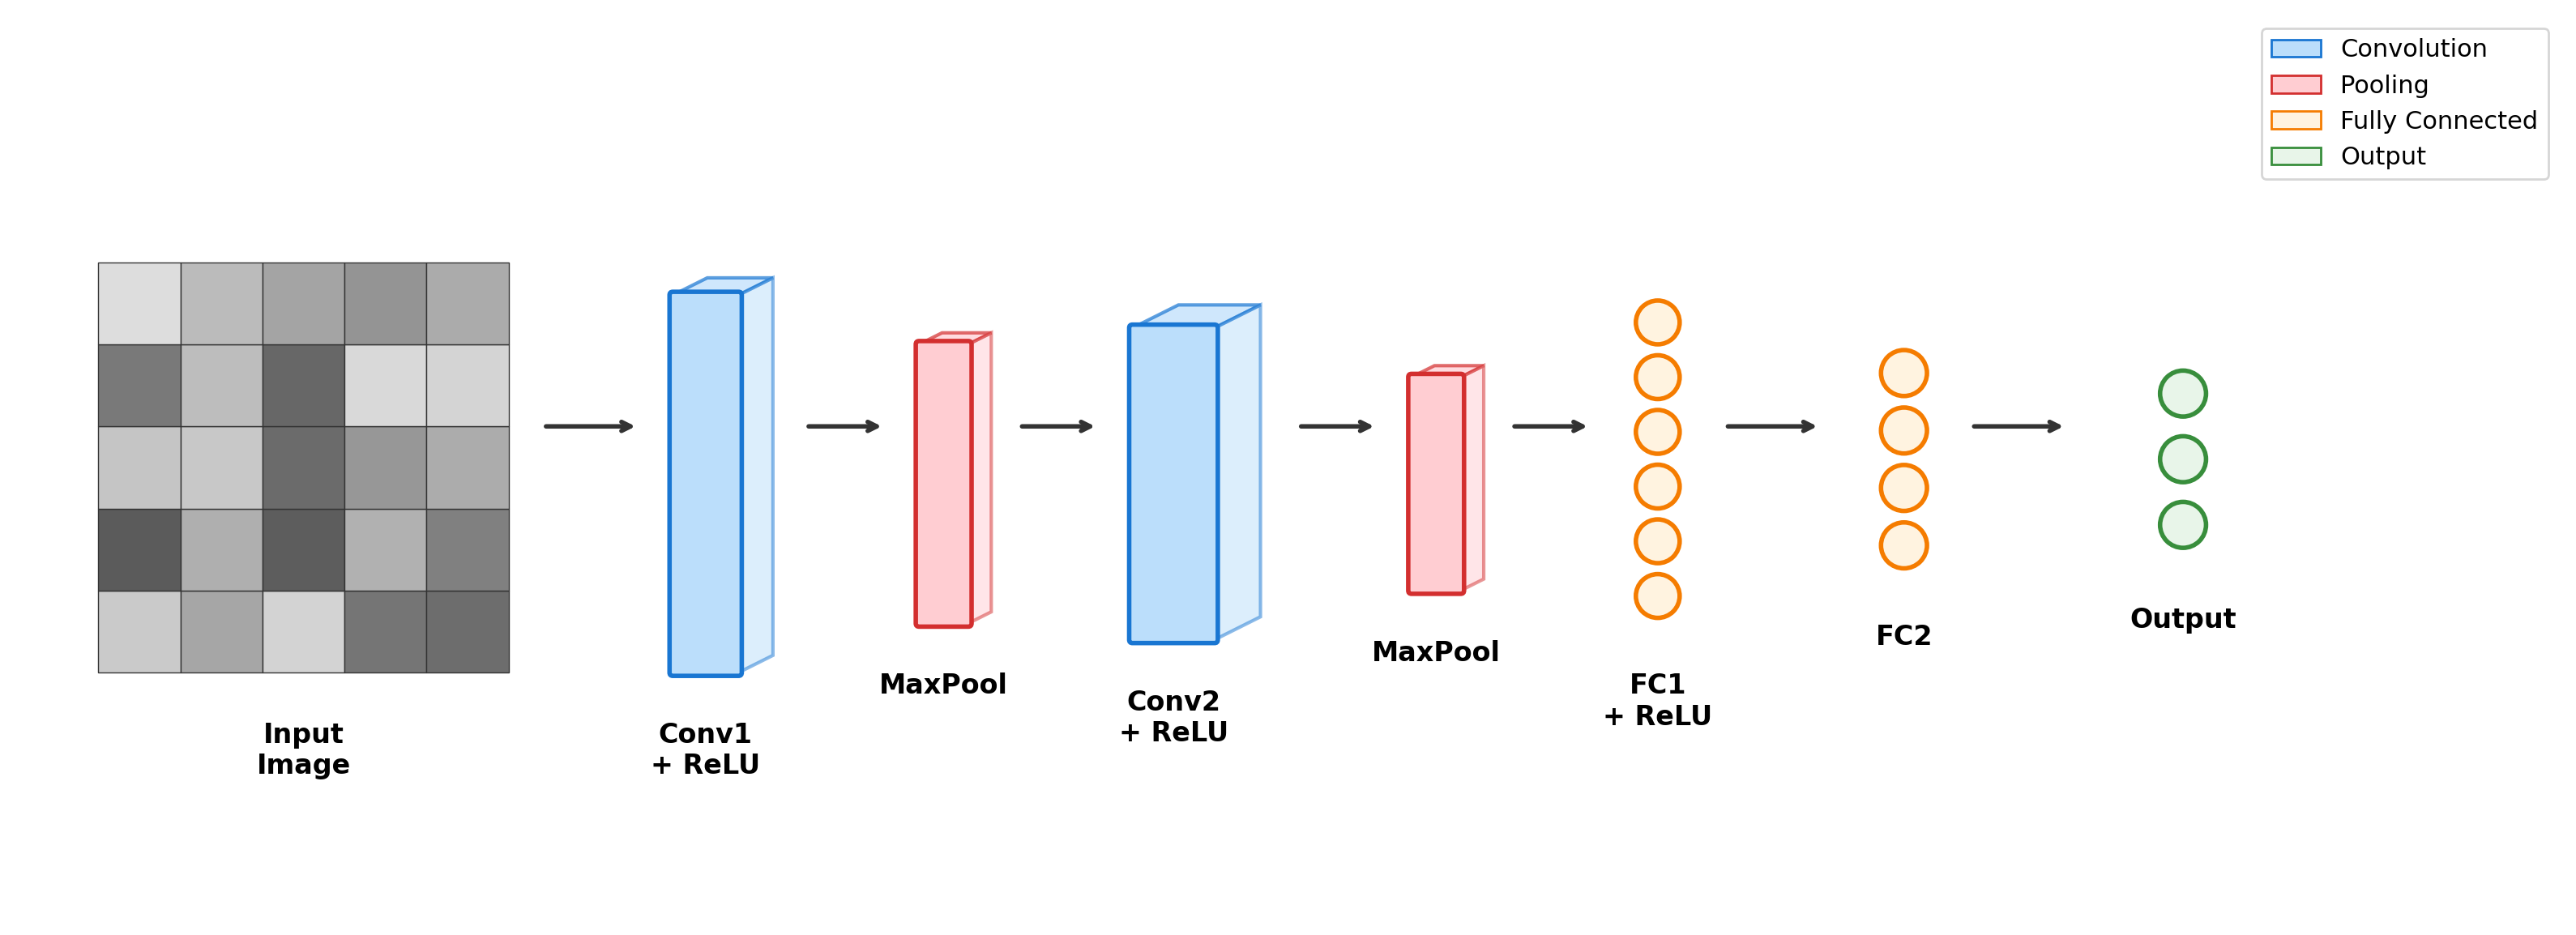
\includegraphics[width=0.95\textwidth]{figures/cnn_architecture.png}
    \end{center}
    
    \vspace{0.5em}
    \textbf{Key components:}
    \begin{itemize}
        \item \textbf{Convolutional layers:} learnable filters/kernels
        \item \textbf{Pooling layers:} downsample spatial dimensions
        \item \textbf{Fully connected:} classification at the end
    \end{itemize}
\end{frame}

% The CNN Solution
\begin{frame}{The CNN Solution: Key Ideas}
    \textbf{1. Local connectivity}
    \begin{itemize}
        \item Small filter (e.g., 3×3) slides across the image
        \item Detects local patterns: edges, textures, curves
    \end{itemize}
    
    \vspace{0.5em}
    \textbf{2. Weight sharing}
    \begin{itemize}
        \item Same filter weights applied at every position
        \item Drastically reduces parameters
        \item Translation invariance built in
    \end{itemize}
    
    \vspace{0.5em}
    \textbf{3. Pooling}
    \begin{itemize}
        \item Downsample and retain dominant signal
        \item Reduces spatial dimensions progressively
    \end{itemize}
    
    \vspace{0.5em}
    \textbf{The kernel weights are learned during training}
\end{frame}

% Learned Kernels
\begin{frame}{What Do Learned Kernels Look Like?}
    \begin{center}
        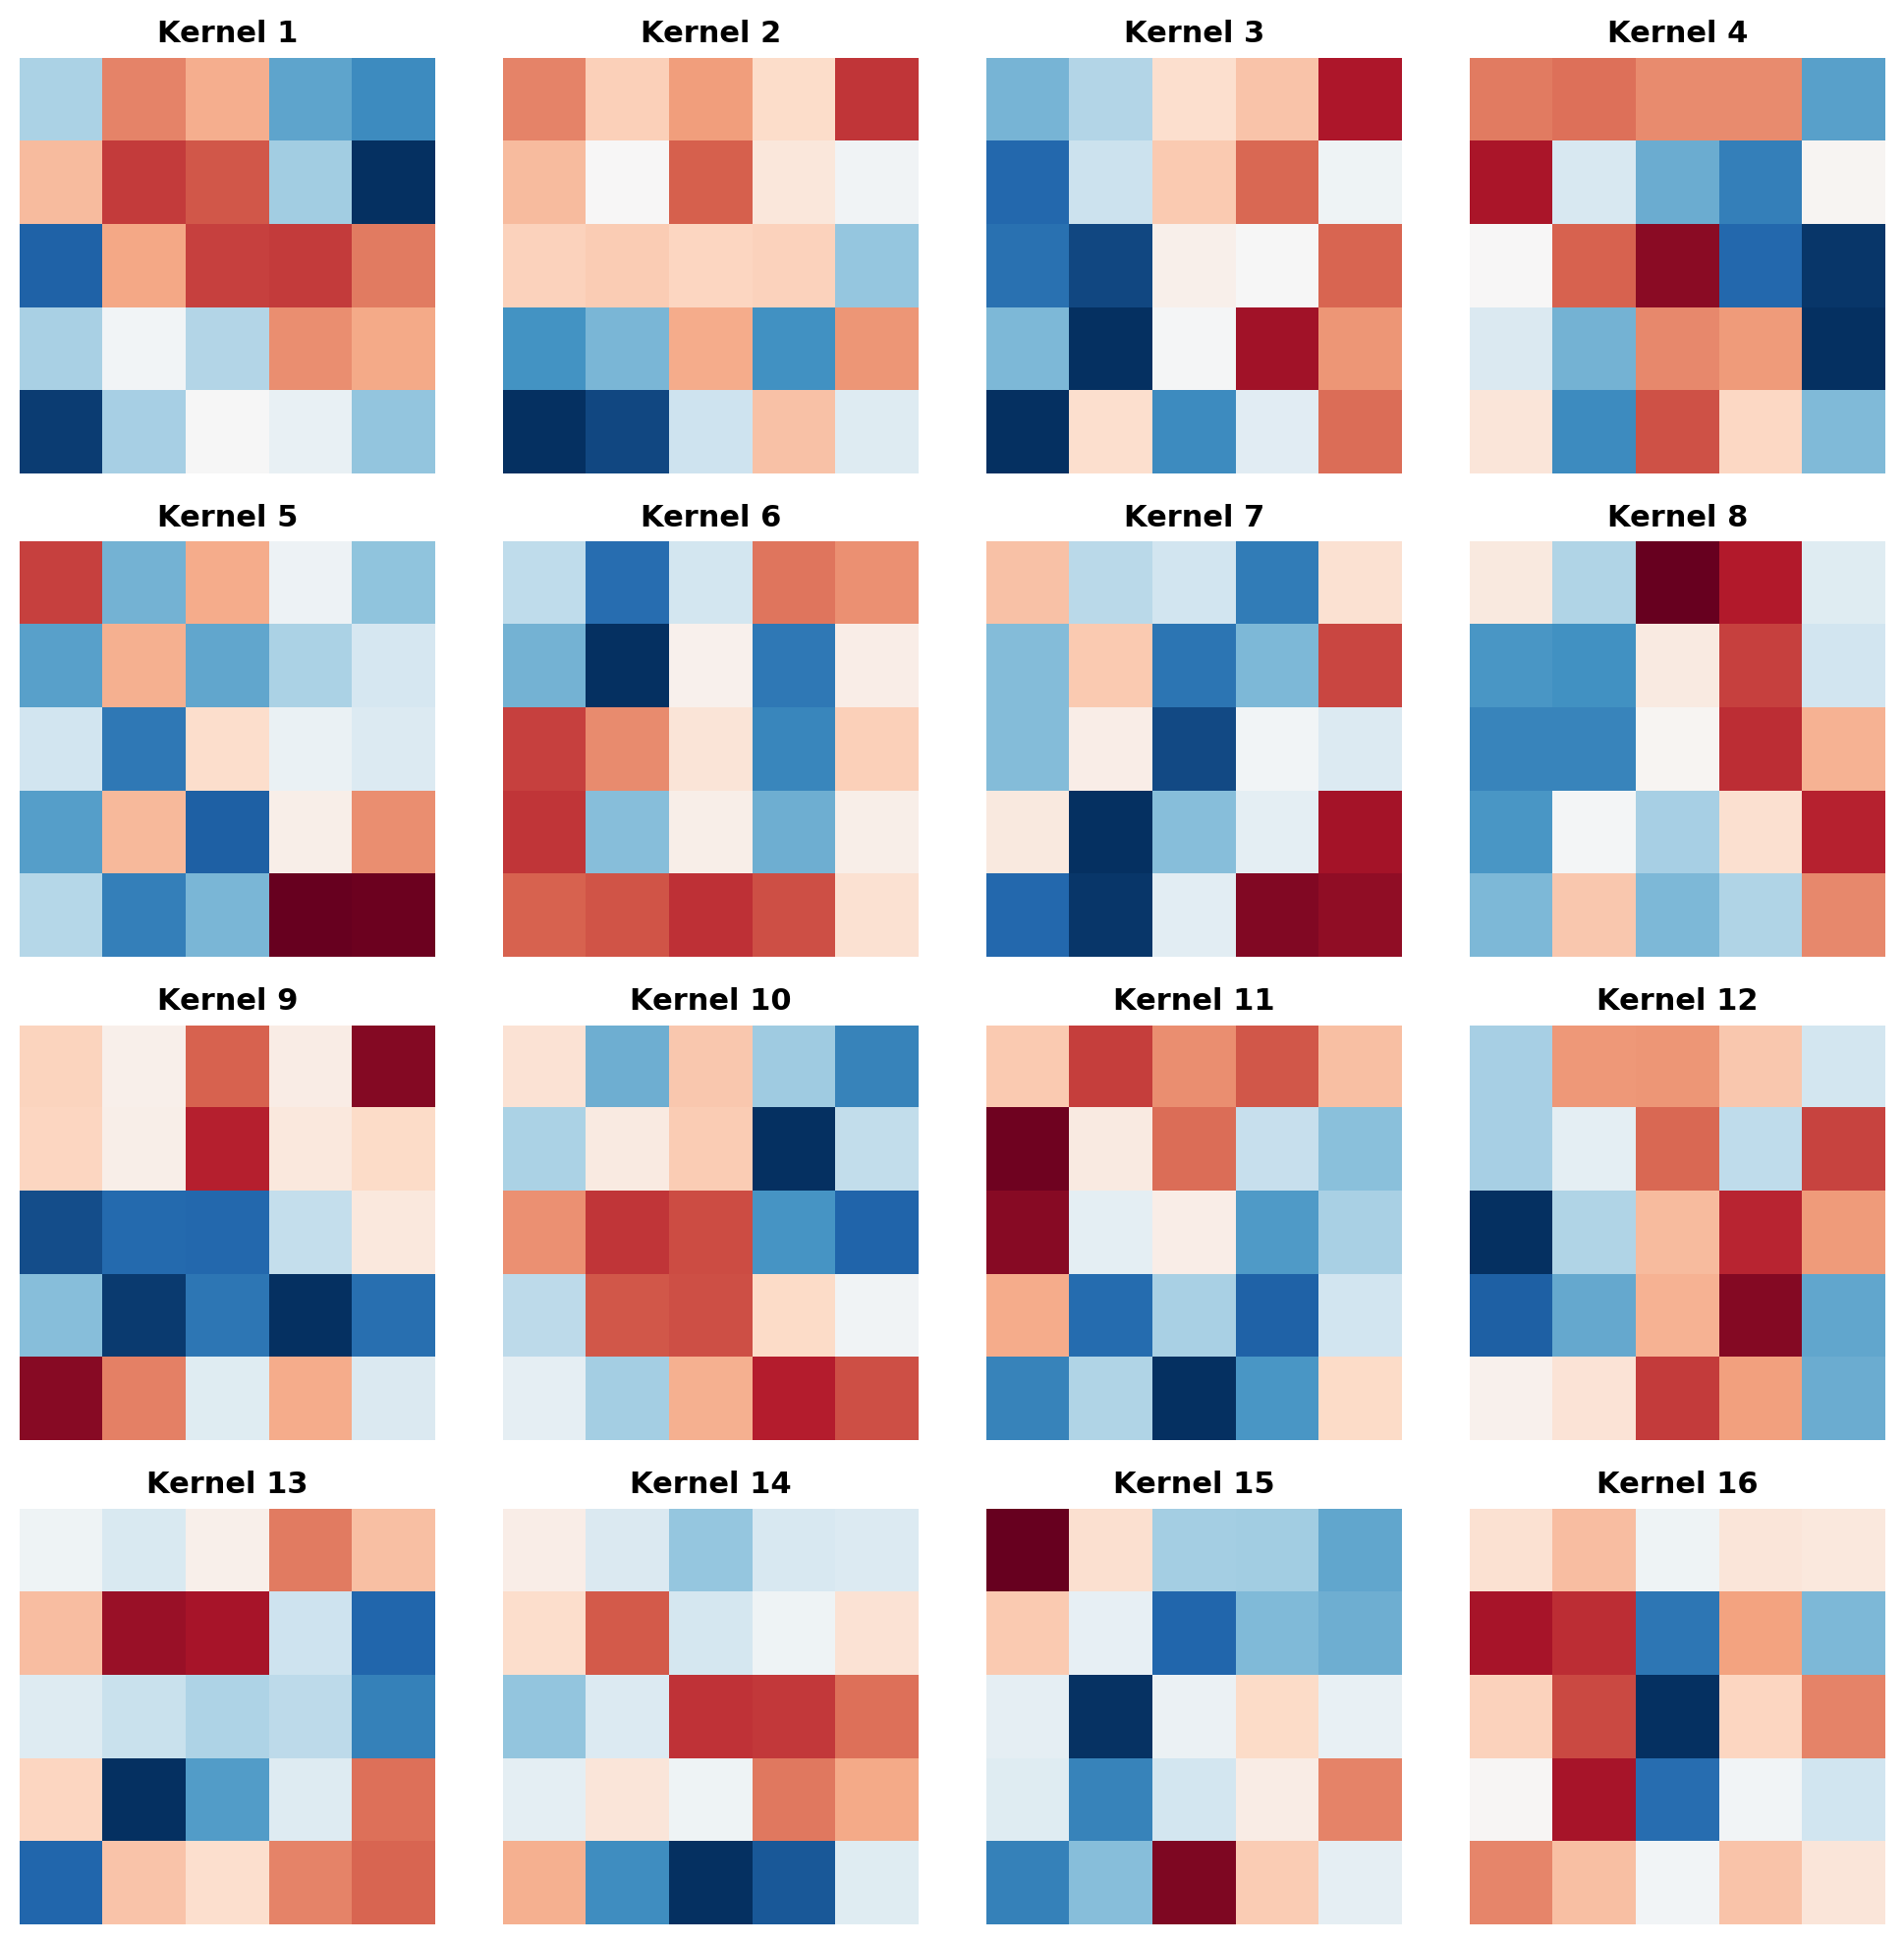
\includegraphics[width=0.7\textwidth]{figures/cnn_kernels.png}
    \end{center}
    
    \vspace{0.5em}
    \textbf{First layer kernels typically learn:}
    \begin{itemize}
        \item Edge detectors (horizontal, vertical, diagonal)
        \item Color blobs
        \item Gabor-like filters
    \end{itemize}
    
    \vspace{0.5em}
    \textit{These emerge from training, not hand-designed}
\end{frame}

% Kernel Applied to Image
\begin{frame}{Kernels Applied to Images}
    \begin{center}
        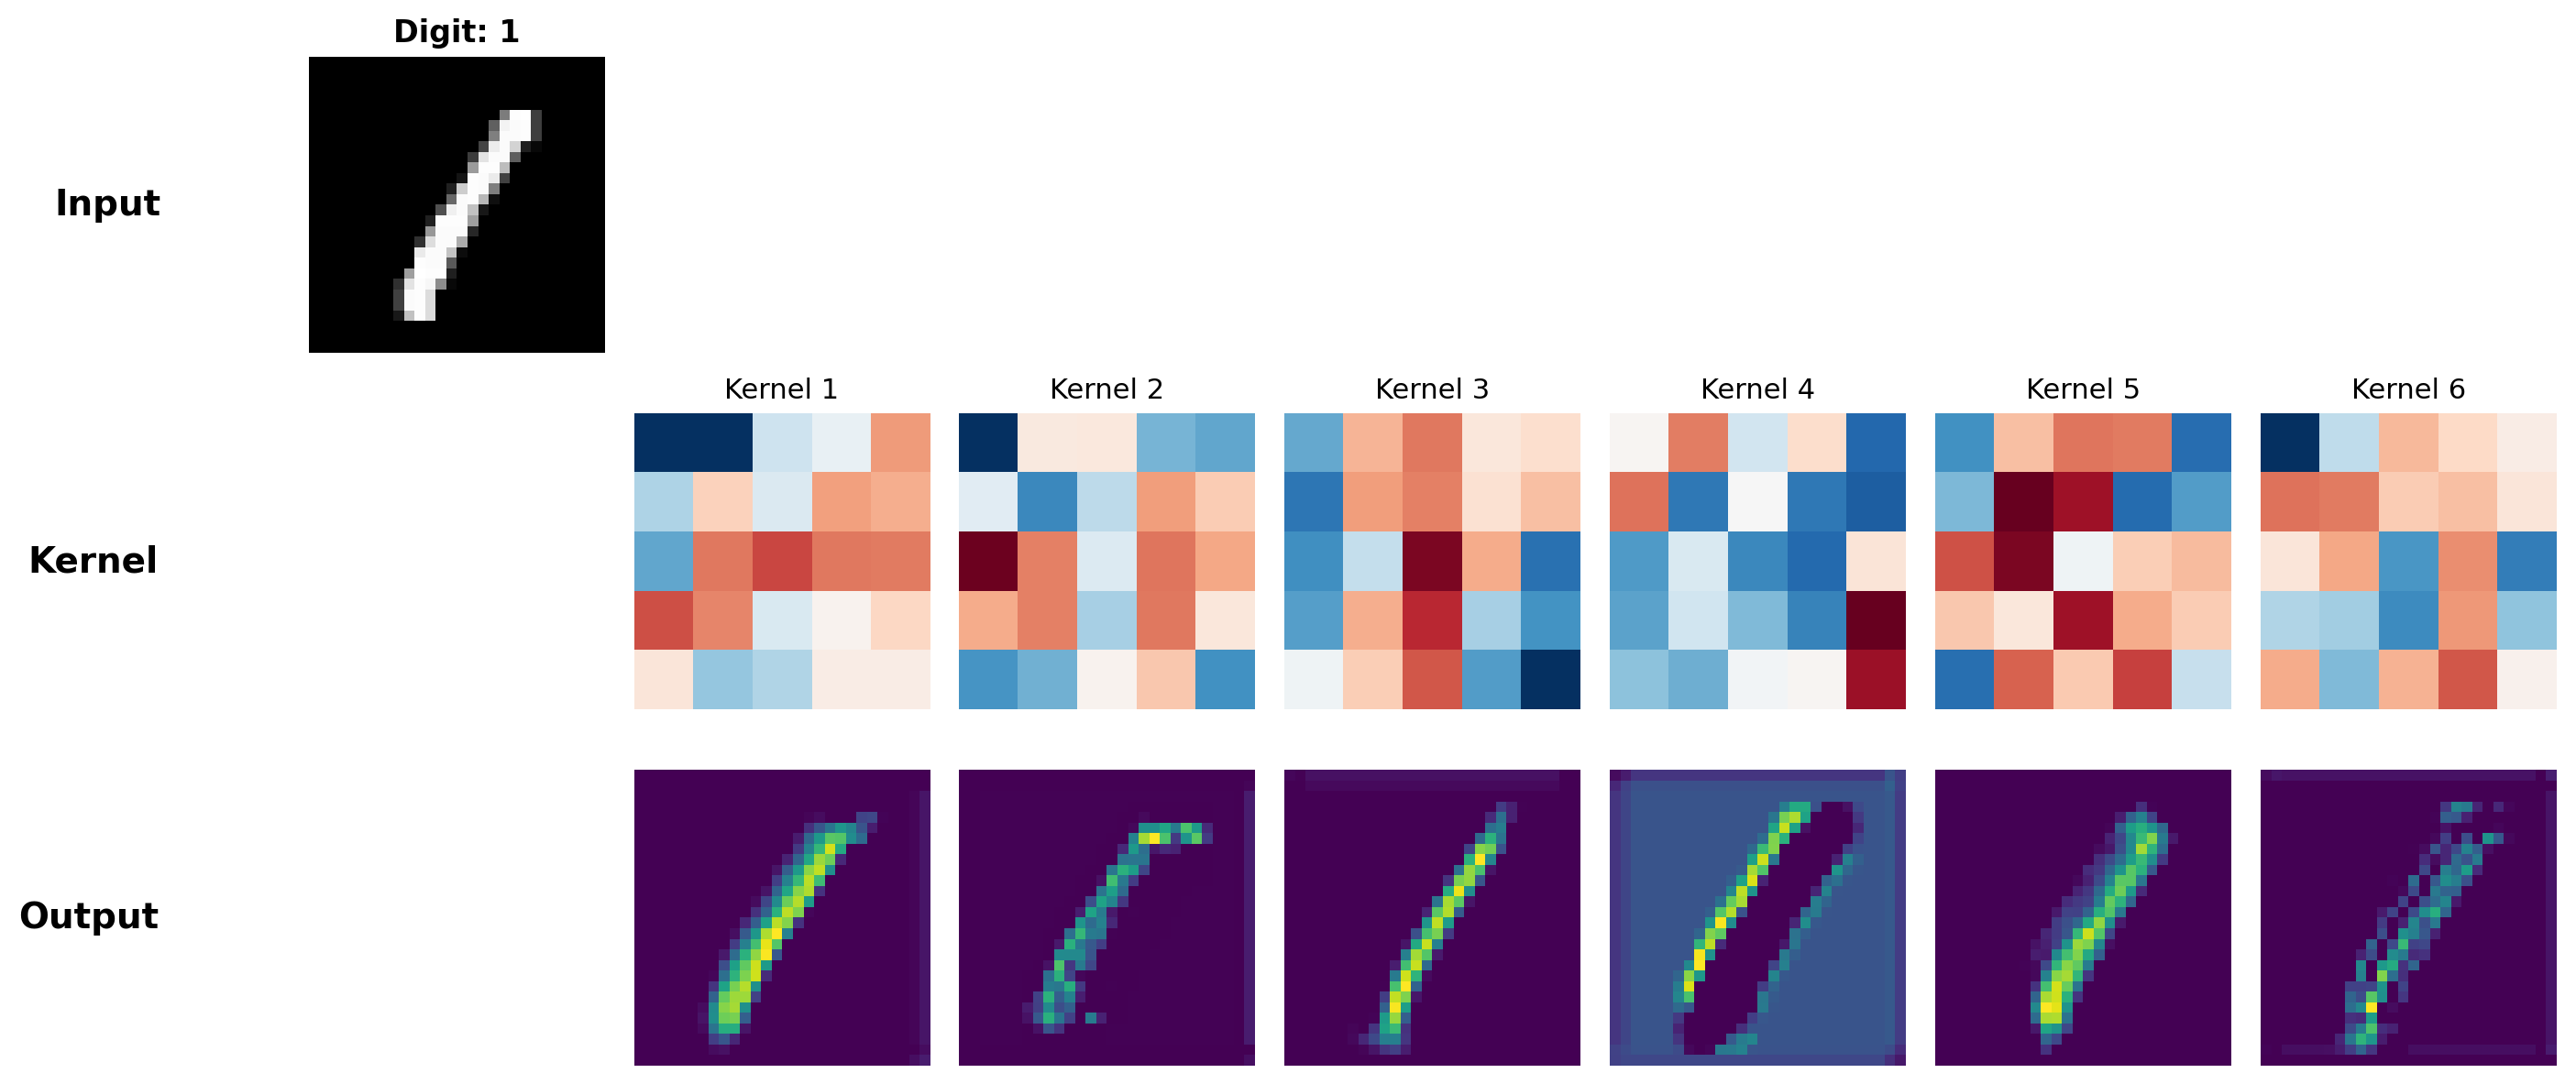
\includegraphics[width=0.95\textwidth]{figures/cnn_kernel_application.png}
    \end{center}
    
    \vspace{0.5em}
    \textbf{Each kernel produces a feature map:}
    \begin{itemize}
        \item Edge kernel $\rightarrow$ highlights edges in image
        \item Stacking layers builds more complex features
    \end{itemize}
\end{frame}

% The Hierarchy
\begin{frame}{CNNs Learn a Hierarchy}
    \textbf{Layer 1:} Edges, gradients, colors
    
    \textbf{Layer 2:} Corners, textures, simple shapes
    
    \textbf{Layer 3:} Parts (eyes, wheels, windows)
    
    \textbf{Layer 4+:} Objects (faces, cars, buildings)
    
    \vspace{1em}
    \begin{center}
        \texttt{Pixels → Edges → Shapes → Parts → Objects}
    \end{center}
    
    \vspace{1em}
    \textbf{This structure emerges from training, not programmed}
\end{frame}

% The Biological Parallel
\begin{frame}{The Biological Parallel}
    \begin{quote}
        ``When ConvNet models and monkeys are shown the same picture, the activations of high-level units in the ConvNet explains half of the variance of random sets of 160 neurons in the monkey's inferotemporal cortex.''
    \end{quote}
    
    \vspace{1em}
    \begin{itemize}
        \item CNNs mirror the hierarchical structure of biological vision
        \item Not designed to; emerged from learning
        \item The visual cortex processes: edges → shapes → objects
    \end{itemize}
\end{frame}

% CNN Commercial History
\begin{frame}{CNNs: Commercial History}
    \textbf{LeCun's work (described without his name):}
    \begin{itemize}
        \item Time-delay neural networks for speech recognition (early 1990s)
        \item Check reading: \textbf{>10\% of all US checks} by late 1990s
        \item Microsoft OCR and handwriting recognition
        \item Face and hand detection in natural images
    \end{itemize}
    
    \vspace{1em}
    \textbf{Then:}
    \begin{quote}
        \small``ConvNets were largely forsaken by the mainstream computer-vision and machine-learning communities until the ImageNet competition in 2012.''
    \end{quote}
    
    \vspace{0.5em}
    \textit{Working for 20 years. Mainstream ignored it.}
\end{frame}

% ImageNet 2012
\begin{frame}{ImageNet 2012: AlexNet}
    \textbf{The result that changed everything:}
    
    \vspace{1em}
    \begin{itemize}
        \item Top-5 error: \textbf{15.3\%} vs runner-up's \textbf{26.2\%}
        \item Not incremental: almost halved the error rate
    \end{itemize}
    
    \vspace{1em}
    \textbf{Key ingredients:}
    \begin{itemize}
        \item GPUs (trained on 2 GTX 580s)
        \item ReLU activation
        \item Dropout regularization
        \item Data augmentation
    \end{itemize}
    
    \vspace{1em}
    \textbf{The field could no longer dismiss deep learning}
\end{frame}

% Looking Forward
\begin{frame}{The Paper's Forward Look (2015)}
    \begin{quote}
        ``Companies such as Mobileye and NVIDIA are using ConvNet-based methods in their upcoming vision systems for cars.''
    \end{quote}
    
    \vspace{1em}
    \textbf{What happened:}
    \begin{itemize}
        \item Tesla Autopilot launched October 2015
        \item NVIDIA pivoted to AI (stock up \textasciitilde20,000\% since 2015)
        \item Every major tech company adopted deep learning
    \end{itemize}
    
    \vspace{1em}
    \textit{The hype was warranted. They knew it would work.}
\end{frame}
